\cleardoublepage
\chapter{中期检查}

\section{项目概况}

本项目初步完成了开发环境搭建,并且开始了调度器的开发与调优工作。

\section{工作进展情况}

\subsection{Kubernetes 环境搭建}

Kubernetes 集群的基本运行需要以下几个部分:

\subsubsection*{etcd}

etcd 的官方描述称之为 etc distributed。即它的功能目标是将 UNIX 系统目录的 /etc 分布式,中心化起来。实际上它的功能与 Apache Zookeeper 类似,是一个分布式高可用的键值对存储服务,或者称为分布式协调服务。在 Kubernetes 当中,一份 k8s 的系统部署会将集群的所有信息持久化在 etcd 当中。所以一套可用的 k8s 部署一定会有一个 etcd 集群。

\subsubsection*{kube-apiserver}

API Server 是用户与 k8s 集群的桥梁,负责接受用户提交的任务,将其持久化并等待调度。

\subsubsection*{kube-controller-manager}

Controller 是 k8s 集群中负责调度某一个应用部署的角色,他们本身需要被一个 Manager 去管理,这个 Manager 也就间接起到了管理整个集群的功能。同样的这个管理者也需要能获取 k8s 集群的部署信息,因此他也需要连接 API Server。可以见得 API Server 一定是承担了以 kubernetes 领域专用的格式和权限管理约定暴露整个集群所有数据的功能。

\subsubsection*{kubelet}

kubelet 是需要部署在受集群管控的每一台机器上的,它是集群 worker 的 agent 角色。kubelet 以 HTTP Server 的方式工作,接受管理者发出的请求来执行命令。

\subsubsection*{kube-proxy}

\subsubsection*{kube-scheduler}

\subsection{快速搭建方式}

因为从零开始搭建 kubernetes 集群可能存在很多细节问题,也有很多条件需求,对域名,网络等等条件都有依赖,且工作量和调试难度都不低。因此这里我们也介绍一下一些已有的工具,用来快速搭建集群。出于不同的目的,两种方式我都进行了尝试。

\subsubsection{Docker in Docker 方法}

\subsubsection{minikube}

在一些基本的配置正确的情况下,minikube 可能是最容易成功运行的方式。尽管如此,这个所谓的“开箱即用”也需要环境满足一些基本要求,例如可以运行 docker-machine。

先在下面给出本人正确运行的方式:

命令行:

\begin{lstlisting}
sudo minikube config set vm-driver none
sudo minikube start
\end{lstlisting}

重要输出:

\begin{lstlisting}
🐳  Version of container runtime is 18.09.2
⌛  Waiting for image downloads to complete ...
E0424 00:19:35.003745    1889 start.go:209] Error caching images:  Caching images for kubeadm: caching images: caching image /root/.minikube/cache/images/gcr.io/k8s-minikube/storage-provisioner_v1.8.1: fetching remote image: Get https://gcr.io/v2/: dial tcp 74.125.204.82:443: i/o timeout
✨  Preparing Kubernetes environment ...
❌  Unable to load cached images: loading cached images: loading image /root/.minikube/cache/images/gcr.io/k8s-minikube/storage-provisioner_v1.8.1: stat /root/.minikube/cache/images/gcr.io/k8s-minikube/storage-provisioner_v1.8.1: no such file or directory
🚜  Pulling images required by Kubernetes v1.14.0 ...
🚀  Launching Kubernetes v1.14.0 using kubeadm ... 
⌛  Waiting for pods: apiserver proxy etcd scheduler controller dns
🔑  Configuring cluster permissions ...
🤔  Verifying component health .....
🤹  Configuring local host environment ...

⚠️  The 'none' driver provides limited isolation and may reduce system security and reliability.
⚠️  For more information, see:
👉  https://github.com/kubernetes/minikube/blob/master/docs/vmdriver-none.md

⚠️  kubectl and minikube configuration will be stored in /root
⚠️  To use kubectl or minikube commands as your own user, you may
⚠️  need to relocate them. For example, to overwrite your own settings:

    ▪ sudo mv /root/.kube /root/.minikube $HOME
    ▪ sudo chown -R $USER $HOME/.kube $HOME/.minikube

💡  This can also be done automatically by setting the env var CHANGE_MINIKUBE_NONE_USER=true
💗  kubectl is now configured to use "minikube"
🏄  Done! Thank you for using minikube!
\end{lstlisting}

下面给出集群启动之后本机所运行的 docker 容器列表。

\begin{lstlisting}
CONTAINER ID        IMAGE                  COMMAND                  CREATED             STATUS              PORTS               NAMES
5d416847c422        5cd54e388aba           "/usr/local/bin/kube…"   20 hours ago        Up 20 hours                             k8s_kube-proxy_kube-proxy-qtctj_kube-system_ba4c62f4-65e3-11e9-9acd-3a4feb33d13b_0
be34a9157d37        k8s.gcr.io/pause:3.1   "/pause"                 20 hours ago        Up 20 hours                             k8s_POD_kube-proxy-qtctj_kube-system_ba4c62f4-65e3-11e9-9acd-3a4feb33d13b_0
6c0e3702a706        k8s.gcr.io/pause:3.1   "/pause"                 20 hours ago        Up 20 hours                             k8s_POD_coredns-fb8b8dccf-tfct6_kube-system_ba4c6fa2-65e3-11e9-9acd-3a4feb33d13b_0
46fb09b54279        k8s.gcr.io/pause:3.1   "/pause"                 20 hours ago        Up 20 hours                             k8s_POD_coredns-fb8b8dccf-ssr52_kube-system_ba4bc787-65e3-11e9-9acd-3a4feb33d13b_0
fde495430bdf        k8s.gcr.io/pause:3.1   "/pause"                 20 hours ago        Up 20 hours                             k8s_POD_storage-provisioner_kube-system_ba4780d4-65e3-11e9-9acd-3a4feb33d13b_0
05e94c674ce5        00638a24688b           "kube-scheduler --bi…"   20 hours ago        Up 20 hours                             k8s_kube-scheduler_kube-scheduler-minikube_kube-system_58272442e226c838b193bbba4c44091e_0
0e0f32af6c4b        ecf910f40d6e           "kube-apiserver --ad…"   20 hours ago        Up 20 hours                             k8s_kube-apiserver_kube-apiserver-minikube_kube-system_267a4c5b83c2f08d16cd0b2fb496fdf3_0
59a4d5ce55c5        2c4adeb21b4f           "etcd --advertise-cl…"   20 hours ago        Up 20 hours                             k8s_etcd_etcd-minikube_kube-system_973c2fad42d1ca0c0cafe14fa28f9a70_0
ad0edb256af6        b95b1efa0436           "kube-controller-man…"   20 hours ago        Up 20 hours                             k8s_kube-controller-manager_kube-controller-manager-minikube_kube-system_6f22129755f0edc1e35623595e40aab2_0
cf7beb5a9f2b        119701e77cbc           "/opt/kube-addons.sh"    20 hours ago        Up 20 hours                             k8s_kube-addon-manager_kube-addon-manager-minikube_kube-system_0abcb7a1f0c9c0ebc9ec348ffdfb220c_0
218f0881a76a        k8s.gcr.io/pause:3.1   "/pause"                 20 hours ago        Up 20 hours                             k8s_POD_kube-scheduler-minikube_kube-system_58272442e226c838b193bbba4c44091e_0
b04d338f0290        k8s.gcr.io/pause:3.1   "/pause"                 20 hours ago        Up 20 hours                             k8s_POD_kube-apiserver-minikube_kube-system_267a4c5b83c2f08d16cd0b2fb496fdf3_0
f7a634bc0085        k8s.gcr.io/pause:3.1   "/pause"                 20 hours ago        Up 20 hours                             k8s_POD_kube-controller-manager-minikube_kube-system_6f22129755f0edc1e35623595e40aab2_0
446a4cd0e374        k8s.gcr.io/pause:3.1   "/pause"                 20 hours ago        Up 20 hours                             k8s_POD_kube-addon-manager-minikube_kube-system_0abcb7a1f0c9c0ebc9ec348ffdfb220c_0
e4d548c62aa5        k8s.gcr.io/pause:3.1   "/pause"                 20 hours ago        Up 20 hours                             k8s_POD_etcd-minikube_kube-system_973c2fad42d1ca0c0cafe14fa28f9a70_0
\end{lstlisting}

因为考虑到要在实体机,云环境,虚拟化等多处运行,为了防止虚拟化环境下缺少嵌套虚拟化支持,我们关闭 minikube 的一切虚拟机后端,设置为 none,即使用本机裸机,并且使用 root 用户 (sudo) 执行命令,从而满足向系统中安装软件的权限限制。这一步可以根据不同的情况进行选择,默认配置的 virtualbox 泛用性较好,在 Linux 环境下,kvm 作为后端也是很好的选择。因为使用 none 裸机环境需要本机具有 docker 环境,读者可以根据自己的环境中具有哪些工具自由选择。

事实上,minikube 同时支持 Windows,macOS,Linux 三大平台,因为主要运行在虚拟机中,系统本机的操作系统环境本身不被依赖。几乎所有主流的虚拟机都被支持,包括了 KVM, VirtualBox, HyperV, VMWare Fusion 等。

下面给出 Kubernetes 集群运行后的 dashboard 截图。

\begin{figure}
    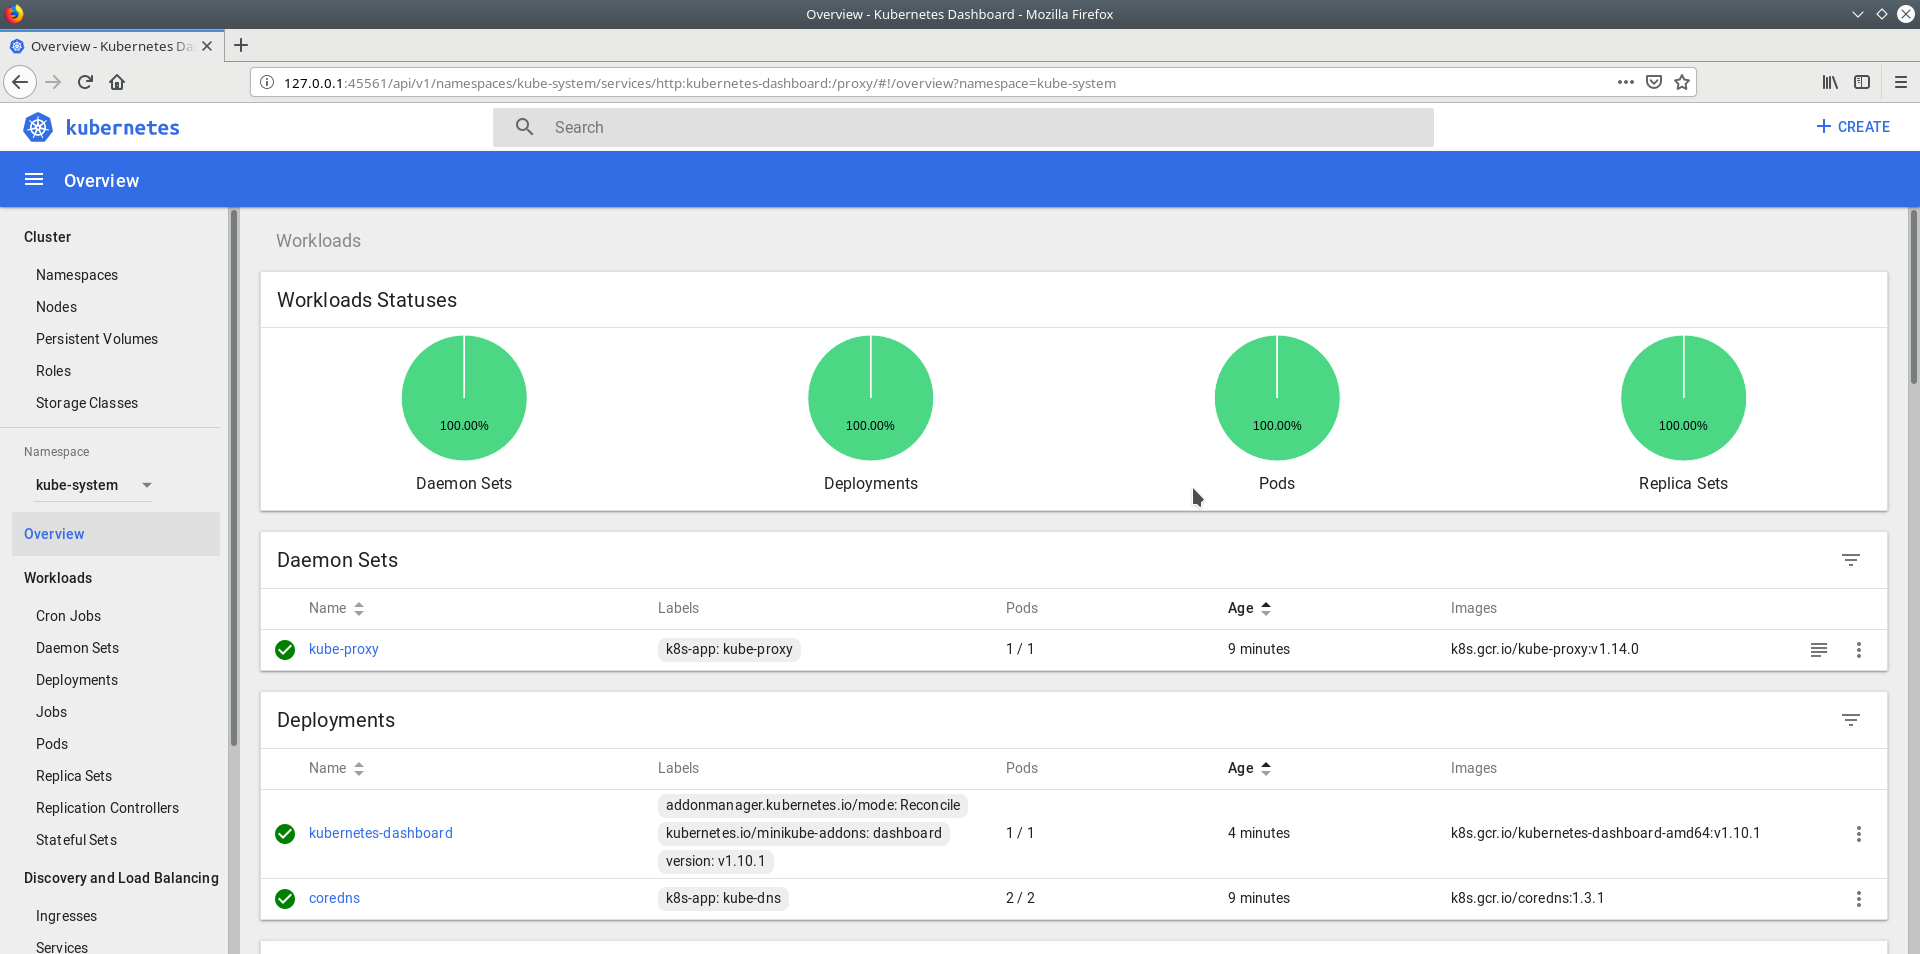
\includegraphics[width=0.8\linewidth]{dashboard-header.png}
    \caption{Kubernetes Dashboard}
\end{figure}

\begin{figure}
    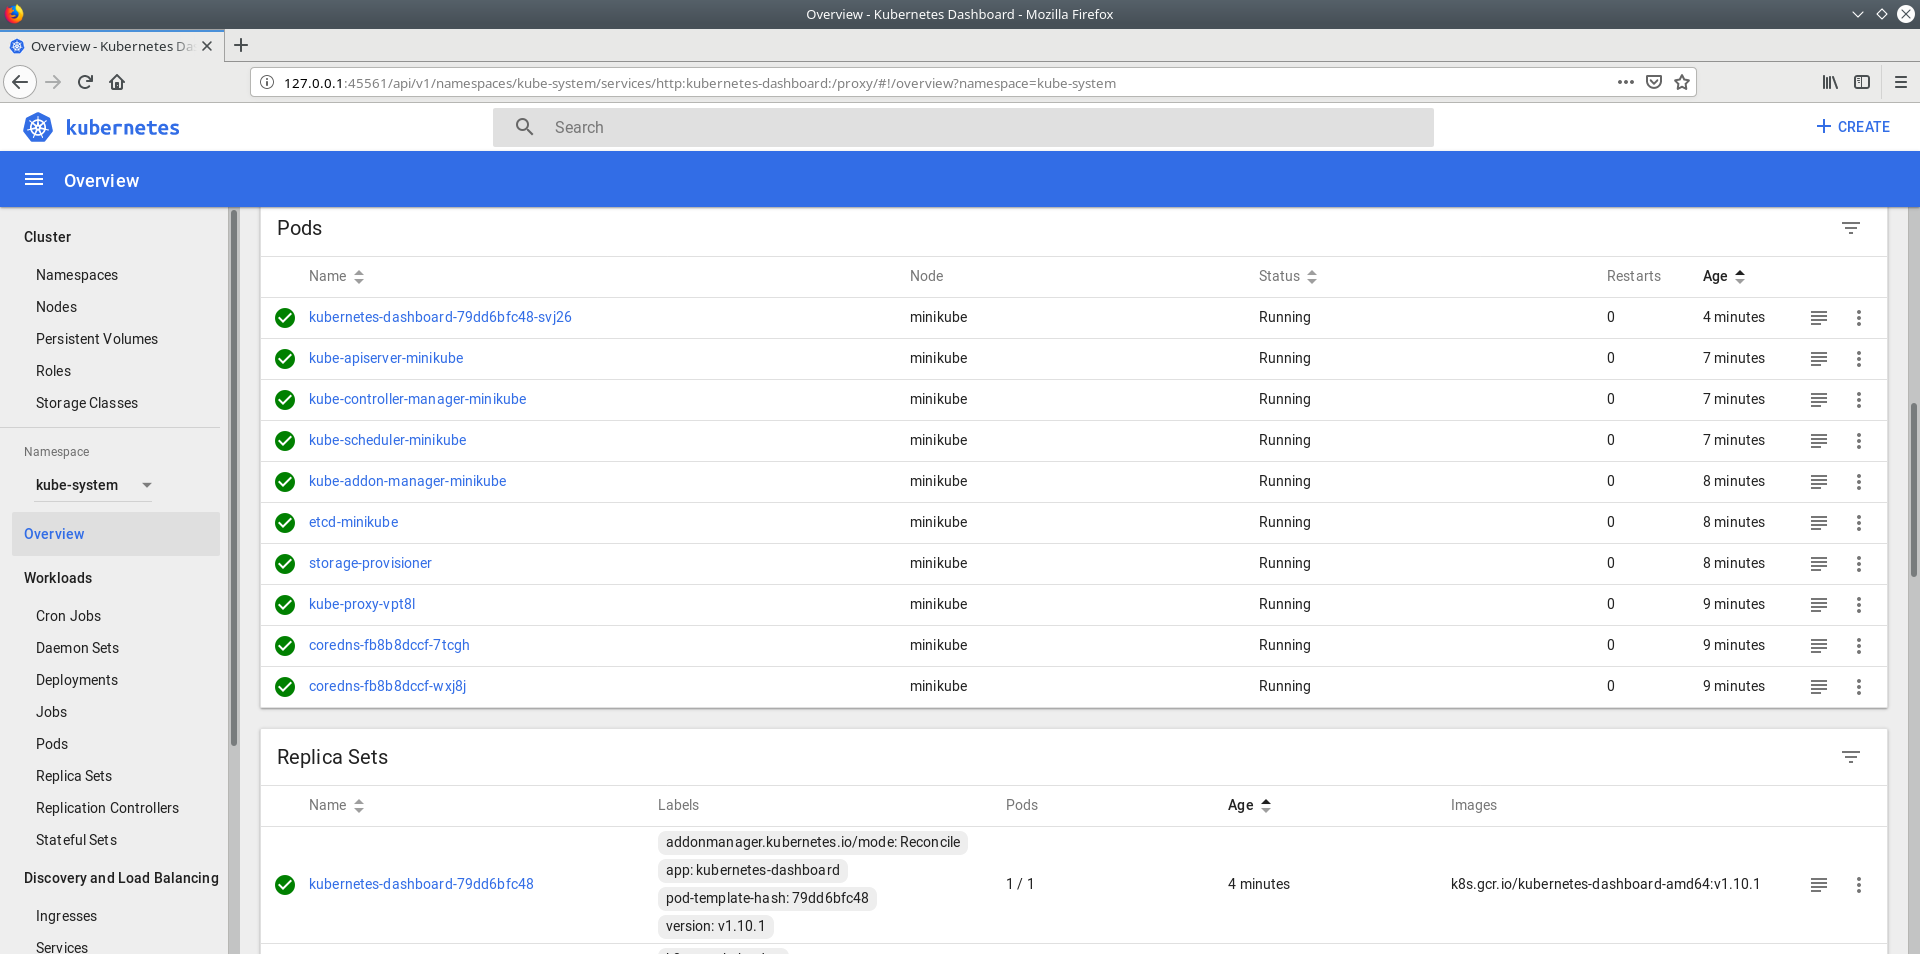
\includegraphics[width=0.8\linewidth]{dashboard-pods.png}
    \caption{Dashboard Pods View}
\end{figure}

尝试在本地 Kubernetes 集群中运行应用:

图中展示了容器编排系统领域的 Hello World,Web 服务器的启动流程。我们在管理页面填写 nginx 镜像的

\begin{figure}
    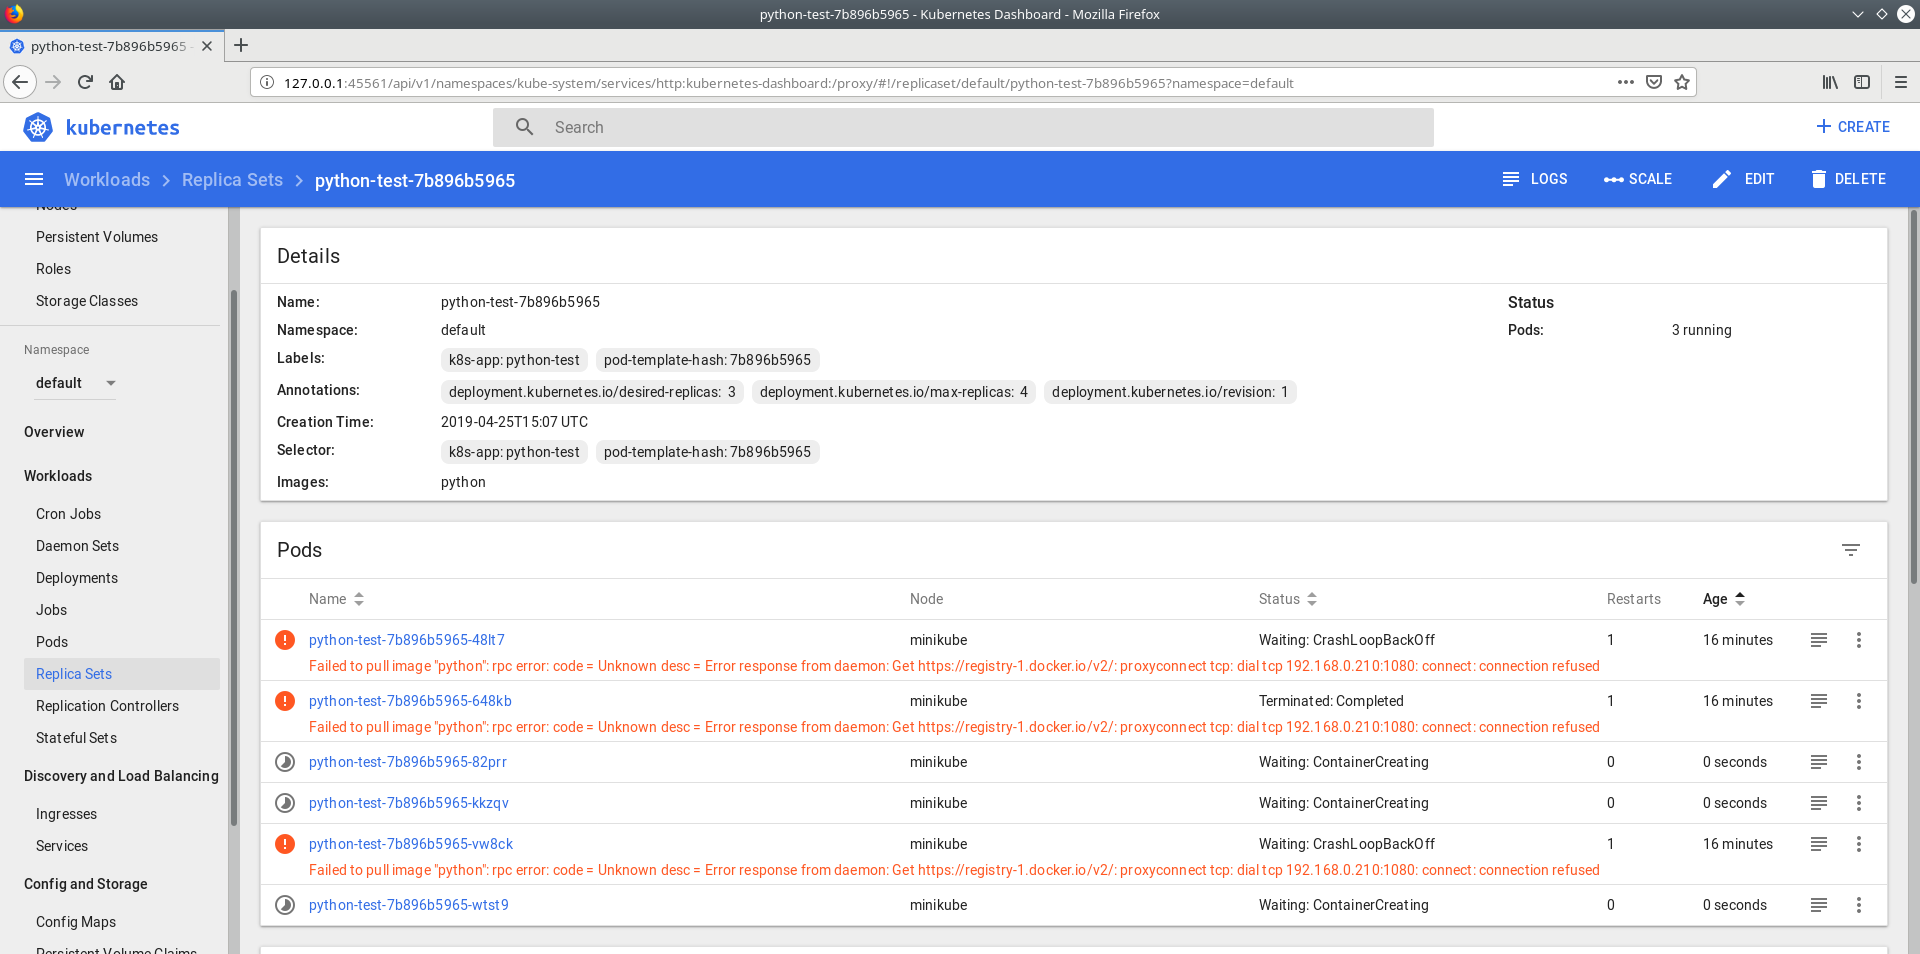
\includegraphics[width=0.8\linewidth]{python-sets.png}
    \caption{Python Replica Set}
\end{figure}

% TODO

\subsection{Operator 开发}

本部分讲述在开发 Operator 的过程,遇到的问题,设计思路以及其中的细节。

Kubernetes 生态的组件多采用 Go 语言开发,Operator 也如此。

开发环境方面,我们使用 GoLand 作为 Go 语言的开发 IDE,使用 gentoo Linux 作为开发环境。使用嵌套虚拟化的方式,在 Linux 虚拟机中运行 KVM 虚拟机作为 Kubernetes 集群的运行环境。

\subsubsection{框架}

Operator SDK 提供了一种快速搭建 Kubernetes Operator 的方法。很容易想到与 API 对接的一个专用角色当中会有很多内容几乎固定的模板代码,SDK 提供的命令行工具可以帮助我们快速生成这部分代码。

https://coreos.com/operators/ 是这个项目的官方网站,可以在这里找到一些说明。总的来讲,Operator 是一种打包,部署和管理 Kubernetes 应用的方法。Kubernetes 应用定义为部署在 Kubernetes 集群中并且使用 Kubernetes API 和 kubectl 工具管理的应用。为了最大化 Kubernetes 的价值,我们应该使用自恰且可解释的 API 对象来描述和管理应用。

\subsubsection{Custom Resource Definition}

\subsection{算法设计}

对于一个通用的调度算法,我们往往可以简化为一个背包问题的延伸。所谓背包问题,指的是我们具有多个背包,每个背包能承载一定量的重量,背包当中需要存放重量各自不同的物品,我们以一个确定的目标,如使用给定的背包数目和规格装下的物品重量之和最大。

对于调度算法来讲,不考虑动态改变配置的场景下调度动作路径的问题,则可以简化为如下一个问题:

对于异质数据和计算逻辑的部署,我们称呼一份数据和计算模型一致的多副本为一个应用(application),承载多个相同应用的一组进程副本为集群(cluster),可见这里的应用就是“物品”,集群就是“背包”。

每个应用有多个不同维度的资源,这是比起传统的背包问题的复杂之处,资源可以包括 CPU 资源,内存,磁盘存储,网络带宽等多个维度。易知在满足这些要求下的优化问题是 NP 完全问题。这意味着

我们需要提供的算法,即是这个场景下的最优化问题。难点在于我们甚至难以给出清晰的最优化定义。在我们的问题中,“背包”的规格,“应用”的规格

\section{问题与建议}

\section{其他}
